\documentclass[master, och, diploma, times]{sty/SCWorks}

\usepackage[T2A]{fontenc}
\usepackage[utf8]{inputenc}
\usepackage{graphicx}
\usepackage{float}

\usepackage[sort,compress]{cite}
\usepackage{amsmath}
\usepackage{amssymb}
\usepackage{amsthm}
\usepackage{fancyvrb}
\usepackage{longtable}
\usepackage{array}
\usepackage[english,russian]{babel}
\usepackage{amsfonts}
\usepackage{commath}
\usepackage{amsthm}

\usepackage[colorlinks=true]{hyperref}

\usepackage{listings}

% для кода
\usepackage{fancyvrb}
\DefineShortVerb{\|}

\theoremstyle{plain}
\newtheorem{thethm}{Теорема}
\newtheorem{lemma}{Лемма}
\newtheorem{note}{Замечание}
\newtheorem{proposition}{Предложение}[section]
\newtheorem{exmp}{Пример}[section]

\theoremstyle{definition}
\newtheorem{defn}{Определение}[section]


\begin{document}

% Кафедра (в родительном падеже)
\chair{дискретной математики}
% Тема работы
\title{Приложение p-адической арифметики к задачам компьютерной алгебры}
% Курс
\course{2}
% Группа
\group{271}
% Специальность/направление код - наименование
\napravlenie{09.03.01 "--- Информатика и вычислительная техника}

% Фамилия, имя, отчество в родительном падеже
\author{Шарова Александра Вадимовича}
% Заведующий кафедрой
\chtitle{к.\,ф.-м.\,н.} % степень, звание
\chname{Л.\,Б.\,Тяпаев}
%Научный руководитель (для реферата преподаватель проверяющий работу)
\satitle{к.\,ф.-м.\,н.} %должность, степень, звание
\saname{Л.\,Б.\,Тяпаев}
% Руководитель практики от организации (только для практики,
% для остальных типов работ не используется)
\patitle{к.\,ф.-м.\,н., доцент}
\paname{Д.\,Ю.\,Петров}

% Год выполнения отчета
\date{2020}

\maketitle
\tableofcontents

\defabbr
\begin{enumerate}
	\item $\mathbb {Z}$ -- кольцо целых рациональных чисел
	\item $\mathbb {Z}_{+}$ -- множество натуральных чисел $\mathbb {N}$
	\item ${N}_0=\{0,1,\dots\}$
	\item $\mathbb {P}$ -- множество простых чисел
	\item Счётное множество -- бесконечное множество, элементы которого возможно пронумеровать натуральными числами.
	\item Плотное множество -- подмножество пространства, точками которого можно сколь угодно хорошо приблизить любую точку объемлющего пространства.
	\item Счётное множество -- бесконечное множество, элементы которого возможно пронумеровать натуральными числами.
	\item Сепарабельное пространство -- топологическое пространство, в котором можно выделить счётное всюду плотное подмножество.
	\item Хаусдорфово пространство — топологическое пространство, удовлетворяющее сильной аксиоме отделимости $T_2$.
	\item Множество из $\mathbb {R}^n$ называется компактом, если из любой последовательности его точек можно выделить сходящуюся подпоследовательность, предел которой принадлежит этому множеству.
	\item Локально компактное пространство — топологическое пространство, у каждой точки которого существует открытая окрестность, замыкание которой компактно.
	\item Размерностью полного метрического пространства $X$ называется наименьшее целое число $n$ такое, что для любого покрытия пространства $X$ существуют вписанное в него подпокрытие кратности $n+1$.
	\item ООП - объектно-ориентированное программирование.
	\item Статический метод - метод который не имеет доступа к данным объекта, и для его использования не нужно создавать экземпляры класса.
\end{enumerate}

\intro
Целью данной магистерской квалификационной работы является ...

Актуальность данной работы обусловлена тем, что

В данной работе будут представлены основные определения и понятия



\section{p-адические числа}

\subsection{p-адическая норма}

\begin{defn}
Пусть $M$ - некоторое непустое множество, и пусть \linebreak ${d: M \times M \rightarrow \mathbb {R}_{\ge0}}$ -- функция двух переменных, определенная на этом множестве и принимающая значения во множестве действительных неотрицательных чисел. Функция $d$ называется метрикой (а множество $M$ -- метрическим пространством), если $d$ удоволетворяет трем условиям:

\begin{enumerate} 
	\item Для каждой пары $a, b \in M$ справедливо: $d(a, b)=0$ тогда и только тогда, когда $a=b$.
	\item Для каждой пары $a, b \in M$ справедливо равенство $d(a, b) = d(b, a)$.
	\item Для каждой тройки $a, b, c \in M$ справедливо неравенство $d(a, b) \le d(a, c) + d(c, b)$.
\end{enumerate}
\end{defn}

\begin{exmp}
Множество $\mathbb {R}$ всех действительных чисел есть метрическое пространство с метрикой $d(a, b)= \abs{a-b}$, где $\abs{.}$ есть абсолютная величина.
\end{exmp}


\begin{defn}
Функция $\norm{.}$, определенная на произвольном коммутативном кольце R и принимающая значения в $\mathbb {R}_{\ge 0}$ называется нормой (также, абсолютной величиной), если она удовлетворяет следующим условиям:

\begin{enumerate} 
	\item Для любого $a \in R$ справедливо, что $\norm{a}=0$ тогда и только тогда, когда $a=0$.
	\item Для каждой пары $a, b \in R$ справедливо равенство $\norm{a \cdot b} = \norm{a} \cdot \norm{b}$.
	\item Для каждой пары $a, b \in R$ справедливо неравенство треугольника: $\norm{a + b} \le \norm{a} + \norm{b}$
\end{enumerate}
\end{defn}

Из определения следует, что если положить $d(a, b)= \norm{a - b}$, то фактически будет задана метрика $d$ на кольце $R$. Данная метрика называется метрикой, индуцированной нормой $\norm{.}$.

\begin{defn}
Пусть $p \in \mathbb {P}$ -- некоторое простое число. В поле $\mathbb {Q}$ введем другую норму $\norm{.}_p$ по правилу:

\begin{enumerate} 
	\item $\norm{0}_p = 0$,
	\item $\norm{n}_p = p ^ {-ord_pn}$,
\end{enumerate}

\noindent где $n > 0$ некоторое натуральное число, а $ord_pn$ показатель степени, в которой число $p$ входит в это произведение. В этом случае норма $\norm{.}_p$ называется $p$-адической нормой.
\end{defn}

Норма $\norm{.}_p$  удовлетворяет всеми характерными свойствами нормы даже в более сильной форме, а именно:

\begin{enumerate} 
	\item $\norm{x}_p \ge 0$, причем $\norm{x}_p = 0$ если $x = 0$.
	\item $\norm{xy}_p = \norm{x}_p \cdot \norm{y}_p$.
	\item $\norm{x + y}_p \le \max(\norm{x}_p, \norm{y}_p)$ \cite{bib:analysis:volovich}
\end{enumerate}

Заметим, что норма $\norm{x}_p$ может принимать лишь счетное число значений $p ^ {-ord_pn}$.

Также, норма $\norm{x}_p$ определяет ультраметрику на $\mathbb {Q}$. Данная норма неархимедова, так как $\norm{nx}_p \le \norm{x}_p \forall n \in \mathbb {Q}_{+}$.

\begin{thethm}
	Нормы $\norm{.}$ и $\norm{.}_p$ $\forall p = 2, 3, \dots$ исчерпывают все нетривиальные неэквивалентные нормы поля рациональных чисел $\mathbb {Q}$.
\end{thethm}


\subsection{Пространство p-адических чисел $\mathbb {Q}_p$}

\begin{defn}
Пополнение поля $\mathbb {Q}$ по $p$-адической норме образует поле $\mathbb {Q}_p$ $p$-адических чисел. Поле $\mathbb {Q}_p$ аналогично полю $\mathbb {R} = \mathbb {Q}_{\infty}$ вещественных чисел, получаемых пополнение поля $\mathbb {Q}$ по норме $\norm{x}=\norm{x}_{\infty}$.
\end{defn}


\begin{defn}
Любое $p$-адическое число $x \ne 0$ однозначно представляется в каноническом виде

\begin{equation} \label{numbers:decomposition}
	x = p^{\gamma} \cdot (x_0 + x_1\cdot p + x_2 \cdot p^2 + \dots
\end{equation}

\noindent где $\gamma = \gamma(x) \in \mathbb {Z}$ и $x_j$ -- целые числа такие, что $0 \le x_j \le p-1$, $x_0 > 0,$ \linebreak $(j=0,1,\dots)$. 
\end{defn}

Представление \eqref{numbers:decomposition} аналогично разложению любого вещественного числа $x$ в бесконечную десятичную дробь:
\begin{equation*}
\begin{aligned}
	x=\pm10^\gamma \cdot (x_0 + x_1 \cdot 10^{-1} + x_2 \cdot 10^{-2} + \dots),\\
	\gamma \in \mathbb {Z}, x_j = 0, 1, \dots, 9, x_0 > 0,
\end{aligned}
\end{equation*}

\noindent и доказывается аналогично.

\begin{proposition}
Пусть $\alpha=p^m(a_0+a_1p+\cdots +a_np^n+\dots)$, где $0 \le a_i \le p$, $a_0 \neq 0$, - $p$ - адическое число. Противоположным к нему является число $- \alpha=\beta=p^m(b_0+b_1p+\cdots+b_np^n+\dots)$, где $b_0=p-a_0$ и $b_i=p-1-a_i$, при $i \geq 0$.
\end{proposition}\label{adic:pros:minus}

Помимо разложения, представление \eqref{numbers:decomposition} дает рациональные числа тогда и только тогда, когда, начиная с некоторого номера числа $x_j, j=0,1,\dots$ образуют периодическую последовательность.

\begin{defn}
Поле $\mathbb {Q}_p$ является коммутативно-ассоциативной группой по сложению;
\end{defn}

\begin{defn}
Поле $\mathbb {Q}_p^*=\mathbb {Q}_p \setminus \{0\}$ является коммутативно-ассоциативной группой по умножению;
\end{defn}

\begin{defn}
Поле $\mathbb {Q}_p^*$ называется мультипликативной группой поля $\mathbb {Q}_p$\cite{bib:analysis:baker};
\end{defn}

\begin{defn}
$p$-адические числа $x$, для которых $\norm{x}_p \le 1$ (т.e. $\gamma(x) \ge 0$ или $\{x\}_p=0$), называются целыми $p$-адическими числами, и их множество обозначается $\mathbb {Z}_p$. Множество $\mathbb {Z}_p$ является подкольцом кольца $\mathbb {Q}_p$; $\mathbb {Z}_+$ плотно в $\mathbb {Z}_p$. Целые числа $x \in \mathbb {Z}_p$, для которых $\norm{x}_p=1$, называютсяются единицами в $\mathbb {Z}_p$. \cite{bib:analysis:vladimirov}
\end{defn}

Совокупность элементов $x$ из $\mathbb {Z}_p$, для которых $\norm{x}_p < 1$ (т.e. $\gamma(x) \ge 0$ или $\norm{x}_p \le \frac{1}{p}$) образуют главный идеал кольца $\mathbb {Z}_p$; Данный идеал имеет вид $p\mathbb {Z}_p$. Поле вычетов $\mathbb {Z}_p \setminus p\mathbb {Z}_p$ состоит из $p$ элементов. В мультипликативной группе поля $\mathbb {Z}_p \setminus p\mathbb {Z}_p$ существует единица $\eta \ne 1$ порядка $p-1$ такая, что элементы $0, \eta, \eta^2, \dots, \eta^{p-1} = 1$ образуют полный набор представителей классов вычетов поля $\mathbb {Z}_p \setminus p\mathbb {Z}_p$.

В силу свойств $p$-адической нормы норма в поле $\mathbb {Q}_p$ удовлетворяет неравенству треугольника:
$$\norm{x + y}_p \le \max(\norm{x}_p, \norm{y}_p) \le \norm{x}_p + \norm{y}_p, x,y \in \mathbb {Q}_p.$$
\noindent Следовательно в $\mathbb {Q}_p$ можно ввести метрику:

\begin{equation}
	\rho (x,y)=\norm{x-y}_p.
\end{equation}

\noindent При этом $\mathbb {Q}_p$ становится полным метрическим пространством. Из представления \eqref{numbers:decomposition} следует сепарабельность $\mathbb {Q}_p$.  

\begin{defn}
$B_{\gamma}(a)$ -- круг радиуса $p^{\gamma^p}$ с центром в точке $a \in \mathbb {Q}_p$:
\begin{equation}
	B_\gamma(a) = \bigg\{x: \norm{x-a}_p \le p^{\gamma} \bigg\}, \gamma \in \mathbb {Z}
\end{equation}
\end{defn}

\begin{defn}
$S_{\gamma}(a)$ -- граница радиуса $p^{\gamma^p}$.
\begin{equation}
	S_\gamma(a) = \bigg\{x: \norm{x-a}_p = p^{\gamma} \bigg\}, \gamma \in \mathbb {Z}
\end{equation}
\end{defn}

\begin{lemma}
Если $b \in B_{\gamma}(a)$, то $B_{\gamma}(b)=B_{\gamma}(a)$.
\end{lemma}

\begin{note}
Круг $B_{\gamma}(a)$ и окружность $S_{\gamma}(a)$ -- открыто-замкнутые множества в $\mathbb {Q}_p$.
\end{note}

\begin{note}
Всякая точка круга $B_{\gamma}(a)$ является его центром.
\end{note}

\begin{note}
Любые два круга в $\mathbb {Q}_p$ либо не имеют общих точек, либо один содержится в другом.
\end{note}

\begin{note}
Всякое открытое множество в $\mathbb {Q}_p$ есть объединение не более чем счетного числа кругов без общих точек.
\end{note}

\begin{lemma} \label{lemma:2}
Если множество $M \subset \mathbb {Q}_p$ содержит две различные точки $a$ и $b$, $a \ne b$, то его можно представить в виде объединения непересекающихся открыто-замкнутых (в $M$) множеств $M_1, M_2$ таких, что $a \in M_1, b \in M_2$.
\end{lemma}

Лемма \eqref{lemma:2} утверждает, что всякое множество пространства $\mathbb {Q}_p$, состоящее из более чем одной точки, несвязно. Другими словами, связная компонента любой точки совпадает с самой точкой. Из этого следует, что $\mathbb {Q}_p$ является вполне несвязным пространством.

Если рассматривать лемму для случая, когда множество $M$ состоит только из двух точек $a$ и $b$, убеждаемся, что существует непересекающиеся окрестности этих точек. Из этого можно сделать вывод, что пространство $\mathbb {Q}_p$ хаусдорфово.

\begin{lemma}
Для того чтобы множество $K \subset \mathbb {Q}_p$ было компактом, необходимо и достаточно, чтобы оно было замкнутым и ограниченным в $\mathbb {Q}_p$
\end{lemma}

\begin{note}
Всякий круг $B_{\gamma}(a)$ является и окружность $S_{\gamma}(a)$ компакты.
\end{note}

\begin{note}
Пространство $\mathbb {Q}_p$ локально компактное.
\end{note}

\begin{note}
Всякий компакт можно покрыть конечным числом кругов фиксированного радиуса без общих точек.
\end{note}

\begin{note}
В пространстве $\mathbb {Q}_p$ справедлива лемма Гейне-Бореля: из каждого бесконечного покрытия компакта $K$ можно выбрать конечное покрытие $K$.
\end{note}

\begin{thethm}
Размерность пространства $\mathbb {Q}_p$ равна $0$.
\end{thethm}

\subsection{p-Адический анализ в $\mathbb {Z}_p$}

Так как компакт $\mathbb {Z}_p$ есть пополнение множества $\mathbb {N}_0$ по метрике \linebreak ${d_p(x,y)=\norm{x-y}_p}$, то любое число из $\mathbb {Z}_p$ есть предел последовательности чисел из $\mathbb {N}_0$.

\begin{defn}
$p$-адическое целое $z$ является пределом последовательности $\{z_i\}^{\infty}_{i=0}$, если если для любого $\epsilon > 0$ найдется $N$ такое, что $\norm{z_i-z}_p < \epsilon$ как только $i>N$. \cite{bib:analysis:anashin}
\end{defn}

\begin{defn}
$p$-адическое целое $z$ есть предел последовательности $\{z_i\}^{\infty}_{i=0}$, если для любого (достаточно большого) положительного рационального целого $K$ найдется $N$ такое, что ${z_i \equiv z \pmod p^K}$ при всех $i>N$. \cite{bib:analysis:anashin}
\end{defn}

\begin{note}
По определению $p$-адической метрики $\norm{z_i-z}_p \le p^{-K}$ тогда и только тогда, когда $z_i \equiv z \pmod p^K$. \cite{bib:analysis:anashin}
\end{note}

\begin{defn}
Функция $f:\mathbb {Z}_p \rightarrow \mathbb {Z}_p$ называется непрерывной в точке $z \in \mathbb {Z}_p$, если для любого (достаточно большого) положительного рационального целого $M$ найдется положительное рациональное целое $L$ такое, что ${f(x) \equiv f(z) \pmod p^M}$ как только $x \equiv z \pmod{p^L}$. \cite{bib:analysis:anashin}
\end{defn}

\begin{defn}
Функция $f$ называется равномерно непрерывной на $\mathbb {Z}_p$, если $f$ непрерывна в каждой точке $z \in \mathbb {Z}_p$, и $L$ зависит только от $M$ и не зависит от $z$.\cite{bib:analysis:ciocan}
\end{defn}


\begin{defn}
Функция $f:\mathbb {Z}_p \rightarrow \mathbb {Z}_p$ называется дифференцируемой в точке $z \in \mathbb {Z}_p$, если существует $p$-адическое число $f'(x) \in \mathbb {Q}_p$ такое, что для любого $M \in \mathbb {N}$ справедливо
\begin{equation} \label{derivative:1}
	\norm{\frac{f(x+h)-f(x)}{h} - f'(x)}_p \le \frac{1}{p^M},
\end{equation}

\noindent если $h$ достаточно мало, т.e. когда $\norm{h}_p \le p^{-K}$, где $K=K(M)$ достаточно велико.
\end{defn}

\begin{defn}
Функция $f$ называется равномерно дифференцируемой (на $\mathbb {Z}_p$), если неравенство \eqref{derivative:1} выполняется одновременно для всех $x \in \mathbb {Z}_p$ как только $h$ достаточно мало. \cite{bib:analysis:anashin:en}
\end{defn}

\begin{lemma}
Если совместимая функция $f:\mathbb {Z}_p \rightarrow \mathbb {Z}_p$ дифференцируема в точке $x \in \mathbb {Z}_p$, то $f'(x) \in \mathbb {Z}_p$.
\end{lemma}

\begin{defn}
Функция $f:\mathbb {Z}_p \rightarrow \mathbb {Z}_p$ называется дифференцируемой в точке $x \in \mathbb {Z}_p$, если существует $p$-адическое число $f'(x) \in \mathbb {Q}_p$ такое, что для любого $M \in \mathbb {N}$ справедливо
\begin{equation} \label{derivative:2}
	f(x+h) \equiv f(x) + h \cdot f'(x) \pmod p^{M + ord_p h}
\end{equation}
\end{defn}

\begin{defn}
Функция $f$ называется равномерно дифференцируемой (на $\mathbb {Z}_p$), если неравенство \eqref{derivative:2} выполняется одновременно для всех $x \in \mathbb {Z}_p$ как только $h$ достаточно мало, т.e. когда $ord_p h \ge K=K(M)$ для достаточно большого $K \in \mathbb {N}$.
\end{defn}

\begin{note}
Правила дифференцирования не зависят от метрики: для вычисления производных суммы, частного и сложной функции в $p$-адическом анализе используются те же формулы, что и в действительном.
\end{note}

\begin{note}
Между действительным и $p$-адическим анализом существует резкое различие например в том, что в и в том, и в в другом случае производная константы равна $0$, однако в $p$-адическом анализе в отличии от действительного равенство нулю производной некоторой функции не означает, что эта функция константа.
\end{note}




% код гензеля
% примеры сложения столбиком и другие операции

\section{Представления $p$-адических чисел и арифметические операции}

\subsection{Представление рациональных чисел в $p$-адической форме}
Пусть $\alpha=\frac{c}{d}$ - рациональное число. Покажем, как найти его $p$-адическое представление. Прежде всего, рассмотрим случай, когда ни $c$, ни $d$ не делятся на $p$. В этом случае $\alpha$ является единицей в поле $p$-адических чисел и может быть записано в виде $\alpha=a_0+a_1p+\cdots+a_np^n+\dots $, где $0 \textless a_0 \textless p$. Значение $a_0$ определяется условием $p \mid (a_0d-c)$ однозначно, поскольку кольцо вычетов по простому модулю является полем и деление на ненулевой элемент в поле всегда возможно и однозначно. Пусть $c-a_0d=c_1p$, $c1 \in \mathbb{Z}$. Тогда $\alpha=a_0+p\frac{c_1}{d}$ и коэффициент $a_1$ однозначно определяется условием $p \mid (a_1d-c_1)$ (он может быть равен нулю). Продолжая этот процесс, мы можем найти любое конечное число цифр в $p$-адическом представлении числа $\alpha$. Для представления чисел, не являющихся $p$-адическими единицами, нужно воспользоваться следующей теоремой:

\begin{thethm}
Всякое отличное от нуля $p$-адическое число $\xi$ однозначно представляется в виде

$$
\xi=p^m(a_0+a_1p^1+\cdots+a_np^n+\dots)
$$

\noindent где $m=\nu_p(\xi)$, $1 \le a_0 \le p-1$, $0 \le a_n \le p-1$$(n=1,2,\dots)$.
\end{thethm}

По аналогии с представлением вещественных чисел в виде бесконечных десятичных дробей, для $p$-адических чисел справедливо следующее утверждение

\begin{proposition}
любое рациональное число может быть представлено в виде переодического $p$-адического числа. Всякое переодическое $p$-адическое число представляет некоторое рациональное число.
\end{proposition}

\subsection{Арифметические операции}

Сложение и умножение $p$-адических чисел выполняется аналогично сложению и умножению десятичных дробей с тем отличием, что цифры складываются или умножаются не справа налево, а слева направо и переносы осуществляются в следующую позицию направо.

\begin{exmp}
Сложить $\frac{2}{3}$ и $\frac{5}{6}$ в $\mathbb{Z}_5$.

\noindent $5$-адическое разложение слагаемых имеет вид

$$
\frac{2}{3}=.4131313\dots
$$
$$
\frac{5}{6}=.0140404\dots
$$
Выполняя сложение, получим

$$
\begin{tabular}{cccccccccccc}
& + & . & 4\; & 1\; & 3\; & 1\; & 3 & 1 & 3 & \dots \\
& = & . & 0\; & 1\; & 4\; & 0\; & 4 & 0 & 4 & \dots \\
\hline
& = & . & 4\; & 2\; & 2\; & 2\; & 2 & 2 & 2 & \dots
\end{tabular}
$$

\noindent Видно, что $5$-адическое представление числа $\frac{2}{3} + \frac{5}{6}=\frac{3}{2}=.4222222\dots$
\end{exmp}

\begin{exmp}
Перемножить $\frac{2}{3}$ и $\frac{5}{6}$ в $\mathbb{Z}_5$.

\noindent $5$-адическое разложение сомножителей имеет вид

$$
\frac{2}{3}=.4131313\dots
$$
$$
\frac{5}{6}=.0140404\dots
$$
Выполняя умножение, получим

$$
\begin{tabular}{ccccccccccccccccc}
& + & . & 4\; & 1\; & 3\; & 1\; & 3 & 1 & 3 & 1 & 3 & 1 & 3 & \dots \\
& = & . & 1\; & 4\; & 0 & 4\; & 0\; & 4 & 0 & 4 & 0 & 4 & 0 & \dots \\
\hline
& & & 4\; & 1\; & 3\; & 1\; & 3 & 1 & 3 & 1 & 3 & 1 & 3 & \dots \\
& & & & 1\; & 2\; & 3\; & 1 & 3 & 1 & 3 & 1 & 3 & 1 & \dots \\
& & & & & & 1\; & 2\; & 3\; & 1 & 3 & 1 & 3 & 1 & \dots \\
& & & & & & & & 1\; & 2\; & 3\; & 1 & 3 & 1 & \dots \\
& & & & & & & & & & 1\; & 2\; & 3\; & 1 &  \dots \\
& & & & & & & & & & & & 1\; & 2\; & \dots \\
\hline
& = & . & 4\; & 2\; & 0 & 1\; & 2\; & 4 & 3 & 2 & 0 & 1 & 2 & \dots \\
\end{tabular}
$$

\noindent Видно, что $5$-адическое представление числа $\frac{2}{3} * \frac{5}{6}=\frac{1}{9}=.4201243201243\dots$
\end{exmp}


Вычитание $p$-адических чисел рекомендуется выполнять в два этапа. Сначала, воспользовавшись предположением \ref{adic:pros:minus}, свести задачу к сложению двух $p$-адических чисел, а затем выполнить это сложение.

\begin{exmp}
Вычесть $\frac{5}{6}$ и $\frac{2}{3}$ в $\mathbb{Z}_5$.

\noindent $5$-адическое представление отрицательного операнда имеет вид

$$
-\frac{5}{6}=.040404\dots
$$

\noindent Выполняя вычитание, получим

$$
\begin{tabular}{cccccccccccc}
& - & . & 4\; & 1\; & 3\; & 1\; & 3 & 1 & 3 & \dots \\
& = & . & 0 \; & 4\; & 0\; & 4 & 0 & 4 & 0 & \dots \\
\hline
& = & . & 4\; & 0\; & 4\; & 0\; & 4 & 0 & 4 & \dots
\end{tabular}
$$

\noindent Видно, что $5$-адическое представление числа $\frac{2}{3} - \frac{5}{6}=-\frac{1}{6}=.04040404\dots$
\end{exmp}


Деление $p$-адических чисел выполняется во-многом аналогично делению столбиком десятичных дробей. Однако, кроме особенности выполнения операций слева направо, отметим еще две: во-первых, вычитание заменяется домножением вычитаемого на $-1$ и последующим сложением, а самое главное, деление является алгоритмическим в том смысле, что первая цифра частного однозначно определяется первыми цифрами делимого и делителя.

\begin{exmp}
Разделить $\frac{2}{3}$ и $\frac{1}{12}$ в $\mathbb{Z}_5$.

\noindent $5$-адическое разложение делимого и делителя имеет вид

$$
\frac{2}{3}=.4131313\dots
$$

$$
\frac{1}{12}=.3424242\dots
$$

\noindent Первой цифрой знаменателя является $3$, обратный к ней элемент в $\mathbb{Z}_5$ - это $2$, т.e. $3^{-1} \equiv 2 \pmod 5$. Следовательно, первая цифра частного равна $4*2 \equiv 3 \pmod 5$. Умножая делитель на $3$, а затем на $-1$, получаем $.111111\dots$. Теперь можем выполнить первый шаг деления столбиком.

$$
\arraycolsep=0.01em
\begin{array}{rrrrrrrr@{\,}r|l}
.&4&1&3&1&3&1&\dots&&\,.3424241\dots\\
\cline{10-10}
&1&1&1&1&1&1&\dots&&\,.3\\
\cline{1-6}
&&3&4&2&4&2&\dots
\end{array}
$$

\noindent Очевидно, что следующей цифрой частного является $1$. Продолжаем деление 

$$
\arraycolsep=0.01em
\begin{array}{rrrrrrrr@{\,}r|l}
.&4&1&3&1&3&1&\dots&&\,.3424241\dots\\
\cline{10-10}
&1&1&1&1&1&1&\dots&&\,.3\\
\cline{1-6}
&&3&4&2&4&2&\dots \\
&&2&0&2&0&2&\dots \\
\cline{1-6}
&&0&0&0&0&0&\dots
\end{array}
$$

в остатке получили $0$, значит деление завершено. В частном мы получили целое число $8$. Легко убедиться, что $\frac{2}{3} \div \frac{1}{12}=8$ и $8=.310000\dots$ в $\mathbb{Z}_5$.

Очевидно, что в общем случае мы ни на каком шаге не получим в остатке $0$. Деление можно продолжать бесконечно. Если делимое и делитель - рациональные числа, что естественно остановиться, как только найдем период частного (который существует, поскольку в этом случае частное также является рациональным числом).

$$
\begin{tabular}{cccccccccccc}
& - & . & 4\; & 1\; & 3\; & 1\; & 3 & 1 & 3 & \dots \\
& = & . & 0 \; & 4\; & 0\; & 4 & 0 & 4 & 0 & \dots \\
\hline
& = & . & 4\; & 0\; & 4\; & 0\; & 4 & 0 & 4 & \dots
\end{tabular}
$$

\noindent Видно, что $5$-адическое представление числа $\frac{2}{3} - \frac{5}{6}=-\frac{1}{6}=.04040404\dots$
\end{exmp}



\subsection{Код Гензеля}
По аналогии с приближением вещественных чисел конечными дробями с фиксированным числом знаков после десятичной (или двоичной, или восьмеричной и т.д.) точки можно рассматривать приближения $p$-адических чисел конечными отрезками их $p$-адического представления с фиксированным числом знаков после $p$-адической точки.

\begin{defn}

Пусть $p$-простое число, $r$-натуральное число и $\alpha=\sum\limits^{\infty}_{i=m} a_ip^i$ - $p$-адическое число ($0 \le a_i \le p, a_m \neq 0$). Кодом Гензеля $p$-адического числа $\alpha$ назовем $p$-адическое представление числа $\sum\limits_{i=m}^{r}a_ip^i$. Для кодов гензеля будем использовать обозначение $H(p,r,\alpha)$, явно содержащее числа $p$, $r$ и $\alpha$. Например, $H(5,4,\frac{1}{3})=.2313$.

\end{defn}

Легко видеть, что если $\alpha$ - рациональное число, то его код Гензеля $\beta=H(p,r\alpha)$ - это такое целое число или несократимая дробь со знаменателем вида $p^k$ для некоторого натурального $k$, что $\alpha-\beta$ представляется несократимой дробью, числитель которой делится на $p^r$. Это условие можно так же обозначить как $\alpha - \beta \equiv 0 \pmod {p^r}$.

Такие коды Гензеля соответствуют представлению вещественных чисел с фиксированной точкой, когда фиксируется абсолютная погрешность представления. Однако существенным отличием $p$-адической арифметики является то, что при сложнении или вычитании чисел абсолютная погрешность не накапливается.

Так же можно ввести понятие кода Гензеля с плавающей точкой. Пусть $\alpha$ - $p$-адическое кольцо. Представим его в виде $\alpha=p^n\epsilon$, где $\epsilon$ - единица кольца целых $p$-адических чисел. В этом случае нормализованным кодом Гензеля с плавающей точкой $\hat H (p, r, \alpha)$ числа $\alpha$ назовем пару $(m_{\alpha}e_{\alpha})$, где $m_\alpha = H(p,r,\alpha)$ и $e_\alpha=n$. Мы назовем $m_\alpha$ мантиссой, а $e_\alpha$ - показателем числа $\alpha$.

Коды Гензеля с плавающей точкой соответствуют представлению вещественных чисел с фиксированной относительной точностью. Снова отметим тот факт, что при умножении кодов Гензеля с плавающей точкой относительная погрешность не накапливается, как это имеет место при умножении вещественных чисел.


\subsection{Примеры операций с кодом Гензеля}

\begin{exmp}
Получить код Гензеля для разности $\frac{3}{4}$ и $\frac{3}{2}$ в $\mathbb{Z}_5$.

\noindent Код Гензеля для операндов имеет вид

$$H(5,4, \frac{3}{4})=(.\; 2\; 1\; 1\; 1,\; 0)$$

$$H(5,4, \frac{3}{2})=(.\; 4\; 2\; 2\; 2,\; 0)$$


\noindent Произведем вычитание

$$
\begin{tabular}{ccccccccccc}
& - & .\; & 2\; & 1\; & 1\; & 1\; & ,\; & 0\; &  \\
& = & .\; & 4 \; & 2\; & 2\; & 2\; & ,\; & 0\; &  \\
\hline
& = & .\; & 3\; & 3\; & 3\; & 3\; & ,\; & 0\; &
\end{tabular}
$$


\noindent Таким образом результатом будет код Гензеля $(.\; 3\; 3\; 3\; 3,\; 0)$, который представляет собой рациональное число $-\frac{3}{4}$.
\end{exmp}


\begin{exmp}
Получить код Гензеля для суммы $\frac{3}{10}$ и $\frac{1}{2}$ в $\mathbb{Z}_5$.

\noindent Код Гензеля для операндов имеет вид

$$H(5,4, \frac{3}{10})=(.\; 4\; 2\; 2\; 2,\; -1)$$

$$H(5,4, \frac{1}{2})=(.\; 3\; 2\; 2\; 2,\; 0)$$


\noindent Поскольку показатели отличаются, мы должны нормализовать код, который имеет больший показатель

$$ 
(.\; 3\; 2\; 2\; 2,\; 0) \rightarrow (.\; 0 \; 3\; 2\; 2\; ,\; -1)
$$

\noindent Теперь мы можем произвести сложение

$$
\begin{tabular}{ccccccccccc}
& - & .\; & 4\; & 2\; & 2\; & 2\; & ,\; & -1\; &  \\
& = & .\; & 0\; & 3\; & 2\; & 2\; & ,\; & -1\; &  \\
\hline
& = & .\; & 4\; & 0\; & 0\; & 0\; & ,\; & -1\; &
\end{tabular}
$$


\noindent Таким образом результатом будет код Гензеля $(.\; 4\; 0\; 0\; 0,\; -1)$, который представляет собой рациональное число $\frac{4}{5}$.
\end{exmp}

\begin{exmp}
Получить код Гензеля для произведения $\frac{4}{5}$ и $\frac{5}{2}$ в $\mathbb{Z}_5$.

\noindent Код Гензеля для операндов имеет вид

$$H(5,4, \frac{4}{5})=(.\; 3\; 3\; 1\; 3,\; -1)$$

$$H(5,4, \frac{5}{2})=(.\; 3\; 2\; 2\; 2,\; 1)$$

\noindent Теперь мы можем произвести умножение

$$
\begin{tabular}{cccccccccc}
& + & .\; & 3\; & 3\; & 1\; & 3\; & ,\; & -1\; \\
& = & .\; & 3\; & 2\; & 2\; & 2\; & ,\; & 1\; \\
\hline
& & & 4\; & 0\; & 0\; & 0\; & & & \\
& & & & 1\; & 2\; & 3\; & & & \\
& & & & & 1\; & 2\; & & & \\
& & & & & & 1\; & & & \\
\hline
& = & . & 4\; & 1\; & 3\; & 1\; & ,\; & 0\; &
\end{tabular}
$$


\noindent Таким образом результатом будет код Гензеля $(.\; 4\; 1\; 3\; 1,\; 0)$, который представляет собой рациональное число $\frac{2}{3}$.
\end{exmp}



%kke 
\begin{exmp}
Получить код Гензеля для частного $\frac{3}{4}$ и $\frac{6}{5}$ в $\mathbb{Z}_5$.

\noindent Код Гензеля для операндов имеет вид

$$H(5,4, \frac{3}{4})=(.\; 2\; 1\; 1\; 1,\; 0)$$

$$H(5,4, \frac{6}{5})=(.\; 1\; 1\; 0\; 0,\; -1)$$

\noindent Теперь мы можем произвести деление и получим код Гензеля $(.\; 2\; 4\; 1\; 3,\; 1)$, который представляет собой рациональное число $\frac{5}{8}$.
\end{exmp}


\section{Разработка однопоточной библиотеки для работы с $p$-адической арифметикой}

Библиотека для работы с $p$-адической арифметикой будет состоять из набора Python модулей, которые представляют из себя единый пакет для пакетного менеджера pip. Данный подход позволит в дальнейшем переиспользовать библиотеку без каких-либо сложностей путем добавления ее в файл requirements.txt. Однопоточная библиотека будет содержать следующие модули:

\begin{itemize}
 
  \item Модуль для работы с $p$-адическими числами. Содержит базовые операции и представляет основные программные интерфейсы. 
  \item Модуль для работы с матрицами. Предоставляет базовые операции над матрицами.
  \item Модуль с алгоритмами, такими как метод Крамера, Гаусса, вычисление определителя.
  \item Модуль с синтетическими тестами, которые используются для сравнения обычных и $p$-адических методов.
 
\end{itemize}


\subsection{Описание типов данных}

Для описания таких типов данных как матрицы и $p$-адические числа был выбран объектно-ориентированный подход. Данный метод позволяет работать с $p$-адическими числами и матрицами как с объектами в классическом понимании, аналогично тому, как мы их представляем в математике. Это позволяет программисту не думать о том, какие методы нужны для работы с теми данными, что он уже определил, так как основная концепция ООП заключается в том, что данные определяются совместно с методами, которые оперируют над ними.


Для описания $p$-адических чисел был реализован Python класс \\ |PAdic(object)|, который предоставляет следующие возможности:

 \begin{itemize}
 
  \item Сложение $p$-адических чисел. Данная операция реализована с помощью метода |__add__|, этот метод является одним из многих т.н. |Magic Methods|, которые позволяют пользователю работать с математическими объектами более естественным образом, а именно использовать знак |+| вместо явного вызова функции которое пользователю может быть неизвестно без подробного ознакомления с библиотекой. Сам метод |__add__| является в свою очередь все лишь оберткой над методом |add_by_offset|, который представляет собой сложение $p$-адических чисел представленных кодом Гензеля.
  \item Вычитание $p$-адических чисел. Данный метод реализован аналогично сложению за исключением того, что использует метод |__sub__|, который в свою очередь является оберткой над методом |subtract_by_offset|.
  \item Вычисление числа со знаком минус. Данная операция реализована с помощью метода |__neg__|. В коде это может быть использовано как: |a = -b|, где |b| это $p$-адическое число.
  \item Вычисление числа со знаком плюс. Данная операция реализована с помощью метода |__pos__|. В коде это может быть использовано как: |a = +b|, где |b| это $p$-адическое число. Данная операция обычно реализуется для симметрии, поскольку унарный минус является оператором, унарный плюс тоже должен быть.
  \item Умножение $p$-адического чисела на целое число. Для данной операции реализован метод |multiply_to_integer|, который является результатом произведения операндов.
  \item Умножение $p$-адических чисел. Для данной операции был использован метод |__mul__|, который нужен для возможности использования знака |*| при работе с числами и представляет собой полноценный метод реализующий $p$-адическое умножение чисел представленных кодом Гензеля.
  \item Деление $p$-адических чисел. Данная операция реализована с помощью метода |__truediv__|, который нужен для возможности использования знака |/| при работе с числами и представляет собой полноценный метод реализующий $p$-адическое умножение чисел представленных кодом Гензеля.
  \item Вычисления порядка $p$-адического числа. Операция реализована методом |calculate_order|. Так как метод статический, то может быть вызван для любого объекта класса из вне с помощью вызова метода \\ |PAdic.calculate_order(a)|, где |a| это $p$-адическое число.
  \item Получение порядка $p$-адического числа. Операция реализована методом |get_order|.
  \item Вывод $p$-адического числа в человеко-читаемом формате. Данная возможность реализована  помощью метода |__str__|. Поскольку функция |print| использует именно функцию |str()| для вывода объекта на экран, то определение метода |__str__| позволит выводить объекты на экран удобным способом: при помощи |print()|.
  \item Вывод $p$-адического числа в виде объекта класса |PAdic|. Данная возможность реализована с помощью метода |__repr__|, который возвращает строку с описанием объекта, которое может быть воспринято итерпретатором языка Python.


  %\item find_multiplier
  %\item do_eratosthene_sieve
  %\item check_for_base_equality
  %\item check_for_prime
\end{itemize}

Для работы с матрицами был реализован собственный Python класс \\ |Matrix(object)|, который позволяет работать не только с обыкновенными типами чисел как например в пакете numpy, но и с $p$-адическими числами. Данный класс предоставляет следующие возможности:
\begin{itemize}
\item Метод |__getitem__| позволяет получать элементы матрицы с помощью классической операции взятия индекса, а именно |A[i][j]|.
\item Метод |__setitem__| позволяет устанавливать элементы матрицы с помощью классической операции работы с индексами, а именно |A[i][j]=2|.
\item Метод для получения ранга матрицы |get_rank|.
\item Метод |reset| - очистка матрицы для дальнейшего переиспользования уже существующего обьекта.
\item Метод |transpose| - транспонирование матрицы. Возвращает $A^{T}$, полученную из исходной матрицы $A$ путем замены строк на столбцы. Оперирует с текущем обьектом.
\item Метод |get_transpose| - получение транспонированной матрицы $A^{T}$ в виде нового объекта, на основании уже существующего объекта.
\item Метод |__add__| реализует возможность складывать матрицы с помощью оператора |+|.
\item Метод |__iadd__| определяет возможность присвоения со сложением с помощью оператора |+=|. Данный метод позволяет использовать конструкцию |A += B|, вместо |A = A + B|.
\item Метод |__sub__| реализует возможность вычитать матрицы с помощью оператора |-|.
\item Метод |__isub__| определяет возможность присвоения с вычитанием с помощью оператора |-=|. Данный метод позволяет использовать конструкцию |A -= B|, вместо |A = A - B|.
\item Метод |__mul__| определяет возможность умножать матрицы с помощью оператора |*|.
\item Метод |__imul__| определяет возможность присвоения с умножением с помощью оператора |*=|. Данный метод позволяет использовать конструкцию |A *= B|, вместо |A = A * B|.
\item Метод |__eq__| реализует возможность сравнения двух матриц с помощью стандартного оператора |=|.
\item Статический метод |make_matrix| заполняет уже сущесвующий объект массивом строк.
\item Статический метод |make_random| возвращает матрицу со случайными значениями.
\item Статический метод |make_zero| возвращает матрицу заполненную нулевыми значениями.
\item Статический метод |make_id| возвращает единичная матрицу $E$, элементы главной диагонали которой равны единице поля, а остальные равны нулю.
\item Вывод матрицы в человеко-читаемом формате. Данная возможность реализована с помощью метода |__str__|. Поскольку функция |print| использует именно функцию |str()| для вывода объекта на экран, то определение метода |__str__| позволит выводить объекты на экран удобным способом: при помощи |print()|.
\item Вывод матрицы в виде объекта класса |Matrix|. Данная возможность реализована с помощью метода |__repr__|, который возвращает строку с описанием объекта, которое может быть воспринято итерпретатором языка Python.

	
\end{itemize}



\subsection{Примеры использования библиотеки}

Так как библиотека основана на объектно-оринтированном подходе и практически все математические операторы перегружены как для матриц, так и для $p$-адических чисел, то использование является достаточно естественным процессом для программиста.


\begin{exmp}
Сложить числа $\frac{3}{2}$ и $\frac{1}{2}$ в $\mathbb{Z}_5$ и вывести представление полученной суммы на экран.
\begin{lstlisting}[language=Python, numbers=left, showstringspaces=false, breaklines=true, basicstyle=\small]
from padic.padic import *
print(PAdic("3/2", 5) + PAdic("1/2", 5))
\end{lstlisting}

\noindent Выводом для данной программы будет число $2$.
\end{exmp}


\begin{exmp}
Сложить числа $\frac{3}{2}$ и $2$ в $\mathbb{Z}_5$ и вывести представление полученной суммы на экран.
\begin{lstlisting}[language=Python, numbers=left, showstringspaces=false, breaklines=true, basicstyle=\small]
from padic.padic import *
print(PAdic("3/4", 5) + PAdic("3/2", 5))
\end{lstlisting}

\noindent Выводом для данной программы будет число $3$, которое в свою очередь представляет собой число $-\frac{3}{4}$.
\end{exmp}


\begin{exmp}
Вычислить определитель матрицы 

$$
\begin{pmatrix}
  1 & 4 \\
  0 & 3 
\end{pmatrix}
$$

\begin{lstlisting}[language=Python, numbers=left, showstringspaces=false, breaklines=true, basicstyle=\small]
from padic.padic import *
from padic.matrix import *
m = Matrix(2, 2)
m1[0] = [PAdic("1", 7),PAdic("4", 7)]
m1[1] = [PAdic("0", 7),PAdic("3", 7)]
\end{lstlisting}

\noindent Выводом для данной программы будет число $3$.
\end{exmp}

\begin{exmp}
Решить СЛАУ методом Крамера

$$
\begin{cases} 
  2x_1 + x_2 + x_3 = 2 \\
  x_1 - x_2 = -2 \\
  3x_1 - x_2 +2x_3 =2
\end{cases} 
$$

\begin{lstlisting}[language=Python, numbers=left, showstringspaces=false, breaklines=true, basicstyle=\small]
from padic.padic import *
from padic.matrix import *
from algo import *
dim = 3
A = Matrix(dim, dim)
A[0] = [PAdic("2", 5), PAdic("1", 5), PAdic("1", 5)]
A[1] = [PAdic("1", 5), PAdic("-1", 5), PAdic("0", 5)]
A[2] = [PAdic("3", 5), PAdic("-1", 5), PAdic("2", 5)]
B = [PAdic("2", 5), PAdic("3", 5), PAdic("3", 5)]
X = cramer(A, B)
\end{lstlisting}

\noindent Выводом для данной программы будет вектор $[.44444, 1, 3]$, где число $(.4444)_5$ представляет собой число $-1$.
\end{exmp}


\begin{exmp}
Решить СЛАУ методом Гаусса

$$
\begin{cases} 
  3x_1 - 2x_2 = -6 \\
  5x_1 + x_2 = 3
\end{cases} 
$$

\begin{lstlisting}[language=Python, numbers=left, showstringspaces=false, breaklines=true, basicstyle=\small]
from padic.padic import *
from padic.matrix import *
from algo import *
dim = 2
A = Matrix(dim, dim)
A[0] = [PAdic("3", 5), PAdic("-2", 5)]
A[1] = [PAdic("5", 5), PAdic("1", 5)]
B = [PAdic("-6", 5), PAdic("3", 5)]
X = gauss(A, B)
\end{lstlisting}

\noindent Выводом для данной программы будет вектор $[0, 3]$.
\end{exmp}





\subsection{Сравнение производительности классических и $p$-адических методов}

\subsubsection{Вычисления опеределителя матрицы}

Для сравнения производительности классического и $p$-адического метода вычисления определителя матрицы вычислим определитель для случайно сгенерированной матрицы $\boldsymbol{A}$, где коэффициенты вычисляются следующим образом:
$$
a_{i,j}= 
\begin{cases} 
1-\bigg(round\bigg(\frac{i-j}{n}\bigg)\bigg)^2, i \neq j, \\ 
10-round\bigg(\frac{i-j}{n}\bigg), i = j.
\end{cases}
$$

Методы будем тестировать при размере матрицы $n=500$ и числе повторений $m=100$.

Время решения будем измерять по циклу вычисления определителя – без учета предварительной подготовки матрицы $\boldsymbol{A}$.

Разные запуски реализаций решения на ПК дают несколько разное время т.к. ОС периодически отбирает ресурсы от нашей программы для своих нужд. Из нескольких запусков будем записывать минимальное время.

Будем, для наглядности, так же сравнивать различные числа из различных полей, таких как $\mathbb{Z}_2$, $\mathbb{Z}_3$, $\mathbb{Z}_5$, $\mathbb{Z}_7$.

\begin{figure}[H]
\centerline{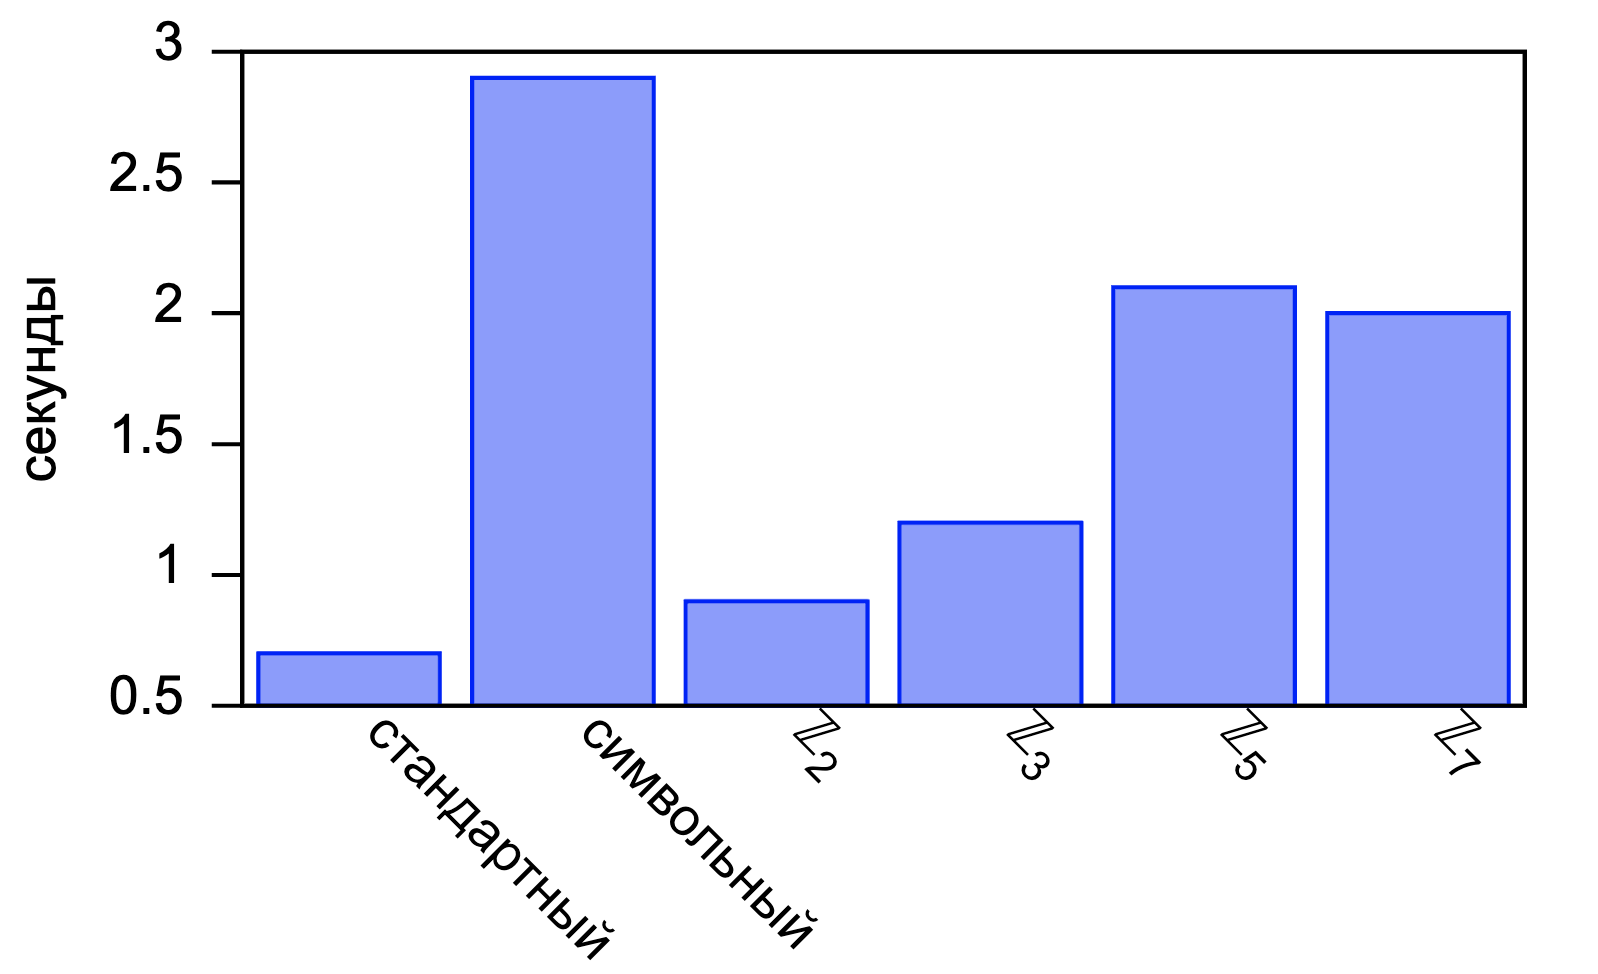
\includegraphics[width=0.85\linewidth]{../gnuplot/single/det/plot.png}}
\caption{todo}
\label{img:single:det}
\end{figure}

Как видно из результатов обычные методы работают немного быстрее, чем $p$-адические методы с числами из $\mathbb{Z}_2$ и $\mathbb{Z}_3$. Время вычисления определителя с числами из $\mathbb{Z}_5$ и $\mathbb{Z}_7$ значительно (в три раза) уступает классическим методам.


\subsubsection{Решение СЛАУ}
Для сравнения производительности классического и $p$-адического метода решения СЛАУ решим $m$ раз систему из $n$ уравнений 

$$
\boldsymbol{A}*\boldsymbol{X}=\boldsymbol{B}
$$

\noindent где $\boldsymbol{A}$ - матрица коэффициентов размером $n \times n$, $\boldsymbol{X}$ - вектор неизвестных и $\boldsymbol{B}$ - вектор правых частей.
Пусть коэффициенты матрицы $\boldsymbol{A}$ вычисляются следующим образом:

$$
a_{i,j}= 
\begin{cases} 
\abs{1-rand(n)*round\bigg(i-j\bigg)^2}, i \neq j, \\ 
10, i = j.
\end{cases}
$$,

\noindent где |rand(n)| некоторое случайное число в диапазоне от $0$ до $n$.

При этом получается симметрическая положительно определенная матрица.
Например, для $n=5$ матрица $\boldsymbol{A}$ будет иметь вид:

$$
\begin{pmatrix}
  10 & 7 & 23 & 53 & 79 \\
  0 & 10 & 8 & 11 & 80 \\
  35 & 2 & 10 & 7 & 11 \\
  17 & 3 & 7 & 10 & 1 \\
  72 & 63 & 11 & 1 & 10
\end{pmatrix}
$$

Пусть на каждом шаге решения $k=1 \dots m$ коэффициенты вектора правых частей равны номеру шага: $b_i = k$.
Чтобы контролировать правильность решения каждым программным средством будем подсчитывать сумму коэффициентов вектора $\boldsymbol{X}$ на каждом шаге решения и суммировать ее по шагам:

$$
S = \sum\limits_{k=1}^{m}\sum\limits_{i=1}^{n} x_i^{(k)}.
$$

Тестировать будем два классических метода решения уравнений - метод Гаусса и метод Крамера.

Оба метода будем тестировать при размере матрицы $n=100$ и числе повторений $m=100$ шагов. При этих параметрах должно получаться $S\approx 224,39195$.

Договоримся, что разложение (факторизацию) матрицы $\boldsymbol{A}$ будем делать на каждом шаге, т.е. каждый раз систему уравнений будем решать полностью.

Время решения будем измерять по циклу решения СЛАУ – без учета предварительной подготовки матрицы $\boldsymbol{A}$.

Разные запуски реализаций решения на ПК дают несколько разное время т.к. ОС периодически отбирает ресурсы от нашей программы для своих нужд. Из нескольких запусков будем записывать минимальное время.

Будем, для наглядности, так же сравнивать различные числа из различных полей, таких как $\mathbb{Z}_2$, $\mathbb{Z}_3$, $\mathbb{Z}_5$, $\mathbb{Z}_7$.
 
\begin{figure}[H]
\centerline{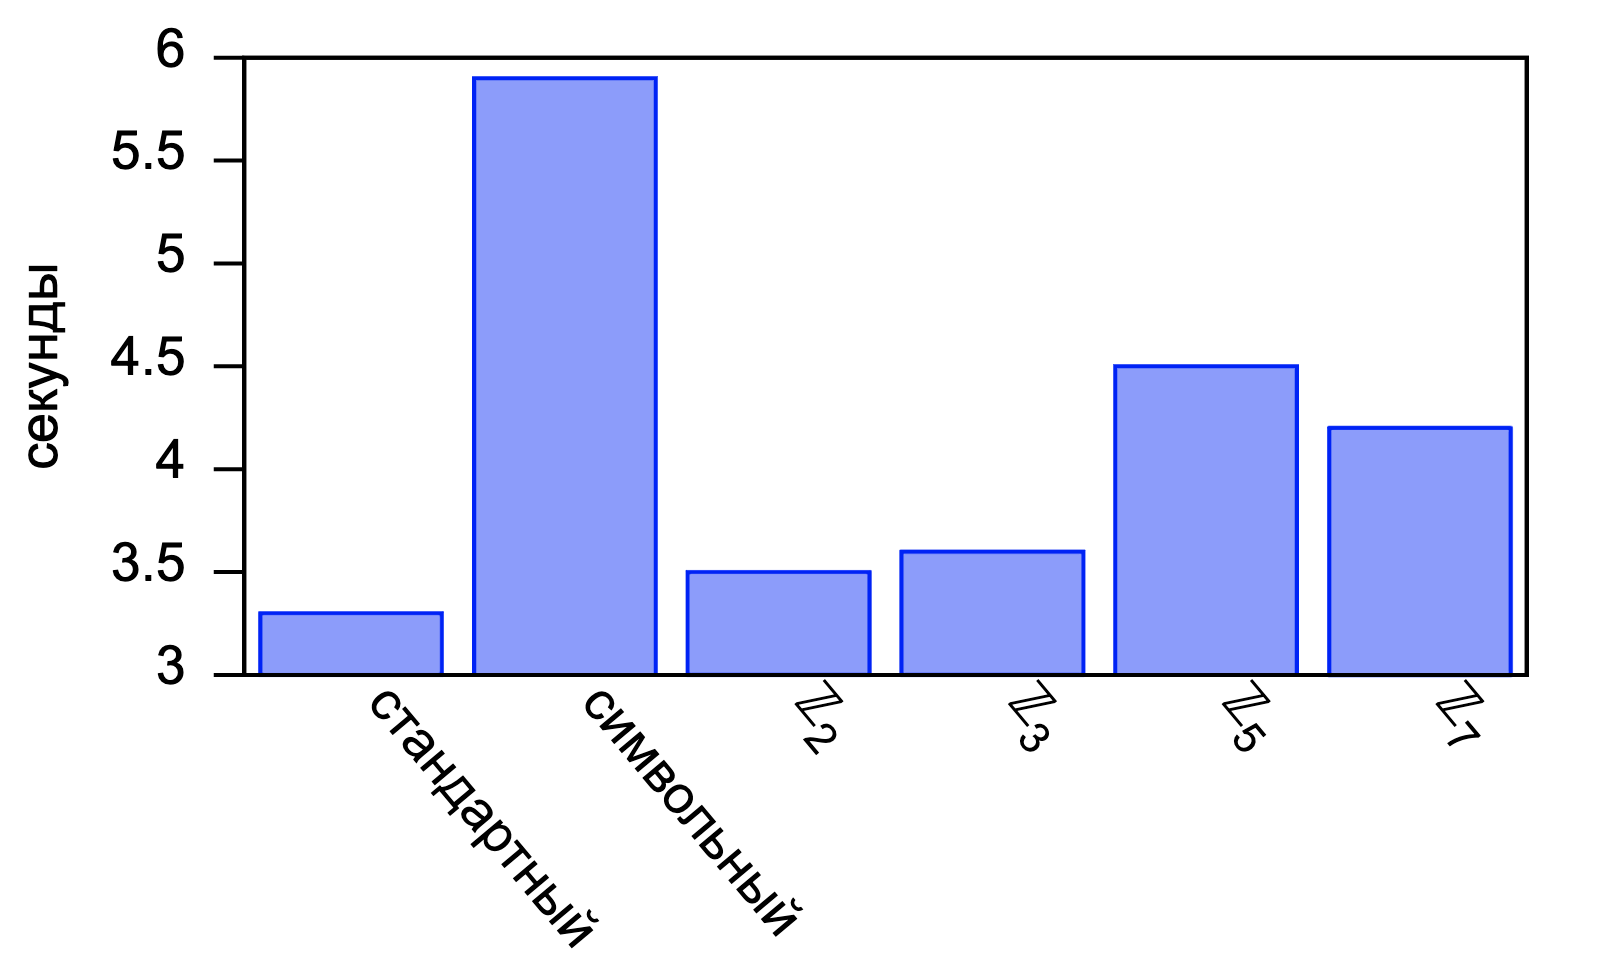
\includegraphics[width=0.85\linewidth]{../gnuplot/single/system_gauss/plot.png}}
\caption{метод Гаусса}
\label{img:single:system}
\end{figure}

\begin{figure}[H]
\centerline{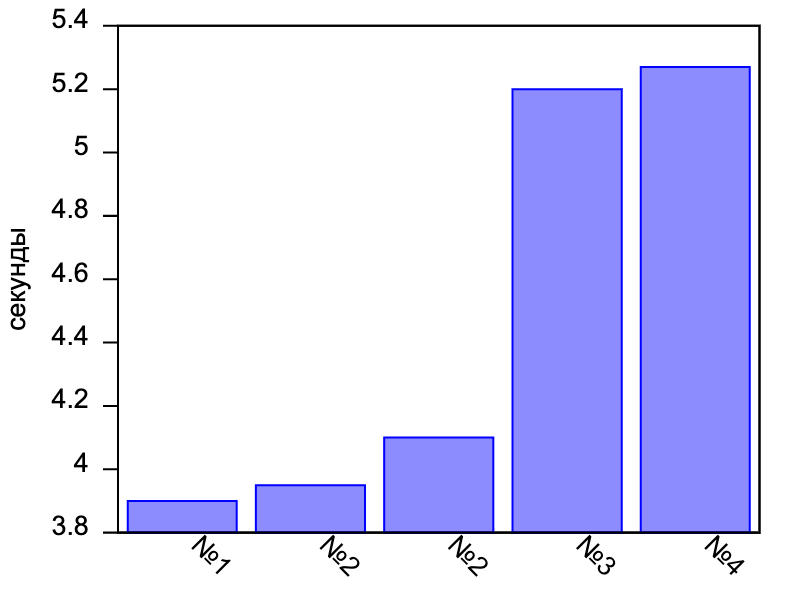
\includegraphics[width=0.85\linewidth]{../gnuplot/single/system_cramer/plot.png}}
\caption{метод Крамера}
\label{img:single:system}
\end{figure}
 
 Как видно из результатов обычные методы работают немного быстрее, чем $p$-адические методы с числами из $\mathbb{Z}_2$ и $\mathbb{Z}_3$. Время решения СЛАУ с числами из $\mathbb{Z}_5$ и $\mathbb{Z}_7$ значительно (в полтора раза) уступает классическим методам.
 
\section{Разработка многопоточной библиотеки для работы с $p$-адической арифметикой}


\begin{figure}[H]
\centerline{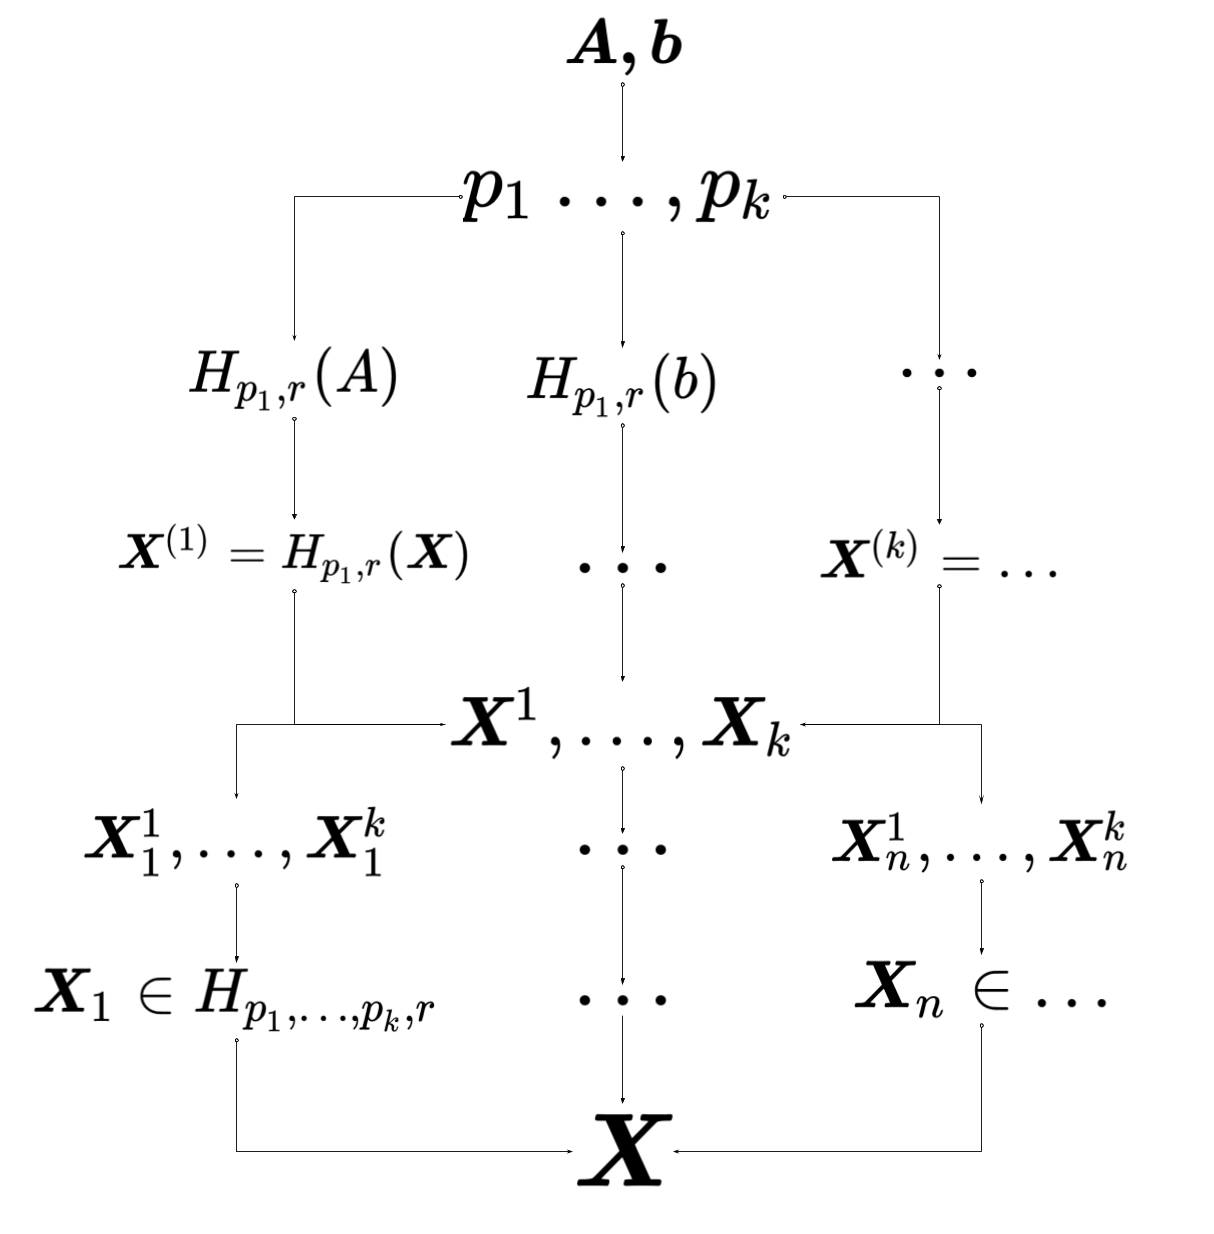
\includegraphics[width=0.7\linewidth]{images/multi/algo.png}}
\caption{Схема параллельного вычисления решения СЛАУ}
\label{img:multi:algo}
\end{figure}




\subsection{Описание алгоритмов для арифметических операций}
\subsection{Сравнение производительности однопоточной и многопоточной библиотеки} 


\section{Сравнение производительности классических и $p$-адических арифметических операций}
\subsection{Решение СЛАУ}
\subsection{Решение ОДУ}
\subsection{Вычисление $e^{Ax}$}


 

\conclusion
В представленной магистерской работе были получены, ...
Реализована возможность ...
В качестве примера были произведены расчеты на различных ...

\bibliographystyle{biblio/ugost}
\bibliography{biblio/biblio}

\appendix

\section{Исходный код библиотеки для работы с $p$-адической арифметикой}

тут будет код


\end{document}